\documentclass{article}
\usepackage{C:/users/fores/math}
\usepackage{xcolor}
\usepackage{amsthm}
\usepackage{graphicx}
\usepackage{hyperref}
\usepackage{natbib}
\newtheorem{theorem}{Theorem}
\newtheorem{lemma}{Lemma}
\newtheorem{remark}{Remark}
\DeclareMathOperator{\softmax}{softmax}
\begin{document}
\title{Initial implementation of implicit transformer}
\author{Forest Yang}
\date{1/9/2023}
\maketitle
\subsection{Defining nonlinearities \texorpdfstring{$\phi_\text{relu}, 
\phi_\text{ln}, T$}{}}
Let $\phi_\text{relu}:\mathbb R^d\to\mathbb R^d$ denote the ReLU activation
applied elementwise, and $\phi_\text{ln}:\mathbb R^d\to\mathbb R^d$ 
the layer normalization transformation (modified by changing the normalization
factor from $\|\tilde x\|_2$ to $\sqrt{1 + \|\tilde x\|_2^2}$ to ensure 
$\phi_\text{ln}$ is 1-Lipschitz)
\begin{equation*}
  \phi_\text{ln}(x) = \frac{\tilde x}{\sqrt{1+\|\tilde x\|_2^2}},\quad
  \tilde x = (I - \frac1d \boldsymbol1\boldsymbol1^\top)x.
\end{equation*}
When given a $d\times n$ matrix, $\phi_\text{relu}$ continues to act 
elementwise, and $\phi_\text{ln}$ acts columnwise: 
\begin{equation*}
  \phi_\text{ln}\left(\begin{bmatrix} x_1 & \ldots & x_n\end{bmatrix}\right)
    = \begin{bmatrix} \phi_\text{ln}(x_1) & \ldots \phi_\text{ln}(x_n)
    \end{bmatrix}.
\end{equation*}
$T:(\mathbb R^{d\times n})^3\to\mathbb R^{d\times n}$
denotes the dot-product attention transformation
\begin{equation*}
  T(X, Y, Z) = Z\softmax_\text{col}\left(\frac1{\sqrt d} X^\top Y\right).
\end{equation*}
\subsection{Lipschitz constants of the nonlinearities}
We use $\|\cdot\|$ on a matrix to denote the max $\ell_2$ norm of any column:
\begin{equation*}
  \|\begin{bmatrix} x_1 & \ldots & x_n\end{bmatrix} \| = \max_{i=1,\ldots,n} \|x_i\|_2.
\end{equation*}
Furthermore, given a linear transformation matrix $A$ we have 
\begin{equation*}
  \max_{X\in\mathbb R^{d\times n},\, \|X\|\leq 1} \|AX\| = 
  \max_{x\in\mathbb R^d,\, \|x\|_2} \|Ax\|_2 = \|A\|_2,
\end{equation*}
the familiar matrix 2-norm, also equivalent to the max singular value.
The Lipschitz constants of $\phi_\text{relu}$ and $\phi_\text{ln}$ are both 1:
\begin{align*}
  \|\phi_\text{relu}(X) - \phi_\text{relu}(Y)\| &\leq \|X - Y\|\\
  \|\phi_\text{ln}(X) - \phi_\text{ln}(Y)\| &\leq \|X - Y\|,
\end{align*}
because in fact, $\|\phi_*(x) - \phi_*(y)\|_2 \leq \|x-y\|_2$ for vectors 
$x$ and $y$ and $*\in\{\text{relu}, \text{ln}\}$.

Now, with $P_{ij} = \frac{\exp(x_i^\top y_j)}{\sum_{l=1}^n \exp(x_i^\top y_l)}$,
and $W^Q, W^K, W^V \in \mathbb R^{p\times d}$,
it may be computed (see Lipschitz constant of self attention paper appendix) that 
\begin{align*}
  \frac{\partial T_i(W^QX, W^KX, W^VX)}{\partial x_j}
  &= \delta_{ij}\frac1{\sqrt p} W^V X P^{(i)} X^\top W^{K^\top} W^Q\\
  &\quad + P_{ij}\frac1{\sqrt p}W^V (x_j - 
  \sum_{l=1}^n P_{il} x_l) x_i^\top W^{Q^\top} W^K\\
  &\quad + P_{ij}W_V, \\
  P^{(i)} &:= \mathrm{diag}\left(\begin{bmatrix} P_{i1} & \ldots & P_{in}
  \end{bmatrix}\right) - \begin{bmatrix} P_{i1} \\ \vdots \\ P_{in}\end{bmatrix}
    \begin{bmatrix}  P_{i1} & \ldots & P_{in}\end{bmatrix}.
\end{align*}
\begin{lemma}
  \label{lem:jaclip}
If for any $H\in\mathbb R^{d\times n}$ with $\|H\|\leq 1$ and
$\|X\|\leq 1$,
\begin{equation}
  \label{eq:jtin}
  \left\|\frac{\partial T_i(W^QX, W^KX, W^VX)}{\partial X} H\right\|_2 
  \leq L,
\end{equation}
then the Lipschitz constant of $X\mapsto T(W^QX, W^KX, W^VX)$ with respect to 
$\|\cdot\|$ is bounded by $L$ for $\|X\|\leq 1$.
\end{lemma}
\begin{proof}
Abbreviating $T_i(X) := T_i(W^QX, W^KX, W^VX)$, for $\|X\|, \|Y\|\leq 1$:
\begin{align*}
  \|T_i(Y) - T_i(X)\|_2 &= \left\|\int_{0}^1 \frac{\partial T_i(X + t(Y-X))}{
  \partial X}(Y-X)\,\mathrm dt\right\|_2 \\
  &\leq \int_0^1 L \|Y-X\| \mathrm dt = L \|Y-X\|
\end{align*}
where we used the fact that $\|X + t(Y-X)\| = \|(1-t)X + tY\| \leq (1-t)\|X\|
+t\|Y\| = 1$. Ergo, $\|T(Y) - T(X)\| \leq L\|Y-X\|$.
\end{proof}
What's left is to find $L$ in \eqref{eq:jtin}, assuming $\|X\|\leq 1$.
\begin{align*}
  &\left\|\frac{\partial T_i(W^Q X, W^KX, W^VX)}{\partial X}H\right\|_2 \\
  &\qquad=
  \bigg\|\frac1{\sqrt p}W^V XP^{(i)}X^\top
  W^{K^\top}W^Q h_i \\
  &\qquad\qquad+\sum_{j=1}^n\big[P_{ij} \frac1{\sqrt p}
  W^V(x_j - \sum_{l=1}^n P_{il}x_l)x_i^\top
  W^{Q^\top} W^Kh_j 
  + P_{ij}W^Vh_j\big]\bigg\|_2 \\
  &\qquad\leq\frac1{\sqrt p}\|W^V\|_2 \|W^K\|_2\|W^Q\|_2 + \frac 1{\sqrt p}
  \|W^V\|_2 \|W^Q\|_2 \|W^K\|_2 + \|W^V\|_2 \\
  &\qquad= \|W^V\|_2\left(\frac2{\sqrt p}\|W^Q\|_2\|W^K\|_2 + 1\right).
\end{align*}
Note if $v$ is a vector with $\|v\|_2\leq 1$, then 
$v^\top XP^{(i)}X^\top v$ is the variance of a r.v. with absolute value 
bounded by 1, and is thus bounded by 1, implying $\|XP^{(i)}X^\top\|_2\leq 1$.
\section{The implicit model}
We divide the state vector into $n_r$ ReLU blocks, $n_l$ layer norm blocks, and $n_a$ 
attention blocks. Then, the implicit model looks like
\begin{align}
&  \begin{bmatrix}
    X_{\text{relu}, 1} \\
    \vdots\\
    X_{\text{relu}, n_r}\\
    X_{\text{ln}, 1} \\
    \vdots \\
    X_{\text{ln}, n_l} \\
    X_{\text{attn}, 1} \\
    \vdots \\
    X_{\text{attn}, n_a}
\end{bmatrix}
= 
  \begin{array}{c}
    \begin{array}{@{}r@{}}
      n_r~\hspace{-1ex}\left\{\begin{array}{c}\null\\\null\\\null\end{array}\right.\vspace{1.5ex}\\
        n_l~\hspace{-1ex}\left\{\begin{array}{c}\null\\\null\\\null\end{array}\right.\vspace{1.5ex}\\
          n_a~\hspace{-1ex}\left\{\begin{array}{c}\null\\\null\\\null\end{array}\right.
    \end{array}
    \hspace{-2ex}
    \left(
    \begin{array}{@{}c@{}}
      \phi_{\text{relu}}\\
      \vdots\\
      \phi_{\text{relu}}\\
      \phi_{\text{ln}}\\
      \vdots\\
      \phi_{\text{ln}}\\
      T\\
      \vdots\\
      T
    \end{array}
    \right)
  \end{array}\nonumber\\
&  \left(
  \begin{bmatrix}
    A^{rr}_{11} & \ldots & A^{rr}_{1n_r} & A^{rl}_{11} & \ldots & A^{rl}_{1n_l} & A^{ra}_{11} & \ldots & A^{ra}_{1n_a}\\
    \vdots & \vdots & \vdots & \vdots & \vdots & \vdots & \vdots & \vdots & \vdots \\
    A^{rr}_{n_r1} & \ldots & A^{rr}_{n_rn_r} & A^{rl}_{n_r1} & \ldots & A^{rl}_{n_rn_l} & A^{ra}_{n_r1} & \ldots & A^{ra}_{n_rn_a}\\
    A^{lr}_{11} & \ldots & A^{lr}_{1n_r} & A^{ll}_{11} & \ldots & A^{ll}_{1n_l} & A^{la}_{11} & \ldots & A^{la}_{1n_a}\\
    \vdots & \vdots & \vdots & \vdots & \vdots & \vdots & \vdots & \vdots & \vdots \\
    A^{lr}_{n_l1} & \ldots & A^{lr}_{n_ln_r} & A^{ll}_{n_l1} & \ldots & A^{ll}_{n_ln_l} & A^{la}_{n_l1} & \ldots & A^{la}_{n_ln_a}\\
    0 & \ldots & 0 & A^{al}_{11} & \ldots & A^{al}_{1n_l} & 0 & \ldots & 0\\
    \vdots & \vdots & \vdots & \vdots & \vdots & \vdots & \vdots & \vdots & \vdots \\
    0 & \ldots & 0 & A^{al}_{n_a1} & \ldots & A^{al}_{n_an_l} & 0 & \ldots & 0
  \end{bmatrix}
  \begin{bmatrix}
    X_{\text{relu}, 1} \\
    \vdots\\
    X_{\text{relu}, n_r}\\
    X_{\text{ln}, 1} \\
    \vdots \\
    X_{\text{ln}, n_l} \\
    X_{\text{attn}, 1} \\
    \vdots \\
    X_{\text{attn}, n_a}
\end{bmatrix}
+ \begin{bmatrix} B_\text{relu} \\ B_\text{ln} \\ 0\end{bmatrix} U + \begin{bmatrix} b_\text{relu} \\ b_\text{ln} \\ 0 \end{bmatrix}
  \right) \label{eq:newimp}
\end{align}
Each entry in the $A$ matrix depicted above is a matrix; for example, $A^{rr}_{ij}$ is a $d_r\times d_r$ matrix, where 
$d_r$ is the dimensionality of a ReLU block, $A^{rl}_{ij}$ is a $d_r\times d_l$ matrix, where $d_l$ is the 
dimensionality of a layer norm block, and $A^{al}_{ij}$ is a $3d_a\times d_l$ matrix, where $d_a$ is the dimensionality
of an attention block. Each $A^{al}_{ij}$ can be divided into $A^{al}_{ij} = (A^{al, Q}_{ij}, A^{al, K}_{ij}, A^{al, V}_{ij})
\in \mathbb R^{3\times d_a\times d_l}$, representing the query, key, and value transformation matrices.
\subsection{Norm matrix of \texorpdfstring{A}{}}
The implicit model \eqref{eq:newimp} satisfies the blockwise lipschitz condition of \citep{idl2019}, where each block is
one of $X_{\text{relu}, i}, X_{\text{ln},j},$ or $X_{\text{ln}, k}$. To each block, we assign the $\|\cdot\|_{2,\infty}$ 
norm, which we define as the maximum 2-norm of any column. Thus, $\|[v_1,\; v_2,\;\ldots,\;v_n]\|_{2,\infty} = 
\max_{i=1,\ldots,n}\|v_i\|_2$.
\subsubsection{\texorpdfstring{$\phi_\text{relu}$}{} and \texorpdfstring{$\phi_\text{ln}$}{} are 1-Lipschitz}
It can be shown that $\phi_\text{relu}$ and $\phi_\text{ln}$ are both 1-Lipschitz with respect to this norm. 
\subsubsection{The Lipschitz constant of attention with layer normed inputs}
For the attention operator $T(X, Y, Z)$, let us show that 
\begin{equation*}
  T\left(\sum_{j=1}^{n_l} A^{al}_{ij} X_{\text{ln}, j}\right) = T\left(\sum_{j=1}^{n_l} A^{al, Q}_{ij} X_{\text{ln}, j},
  \sum_{j=1}^{n_l} A^{al, K}_{ij} X_{\text{ln}, j}, \sum_{j=1}^{n_l} A^{al, V}_{ij} X_{\text{ln}, j}\right)
\end{equation*}
is Lipschitz with respect to $X_{\text{ln}, h}$, for each $h=1,\ldots, n_l$,
using the fact that $\forall j=1,\ldots, n_l,\;\|X_{\text{ln}, j}\|_{2,\infty} \leq 1$ due to
being the output of a layer norm activation.

To control the Lipschitz constant, we compute the Jacobian of $T(\sum_{j=1}^{n_l} A^{al}_{ij}X_{\text{ln}, j})$ with respect
to a specific $X_{\text{ln}, h}$. For short, we denote 
\begin{align*}
\tilde X_i^Q &= \sum_{j=1}^{n_l} A^{al, Q}_{ij} X_{\text{ln},j}\\
\tilde X_i^K &= \sum_{j=1}^{n_l} A^{al, K}_{ij} X_{\text{ln},j}\\
\tilde X_i^V &= \sum_{j=1}^{n_l} A^{al, V}_{ij} X_{\text{ln},j}\\
\tilde X_i &= \sum_{j=1}^{n_l} A^{al}_{ij} X_{\text{ln},j} = 
[\tilde X_i^{Q^\top},\; \tilde X_i^{K^\top},\; \tilde X_i^{V^\top}]^\top.
\end{align*}
Now, we compute the the Jacobian of $T(\tilde X_i)_t$, 
the $t$th column of $T(\tilde X_i) = [T(\tilde X_i)_1,\; \ldots,\; T(\tilde X_i)_n]\in\mathbb R^{p\times n}$,
with respect to $X_{\text{ln}, h}$, times an input $Z = [z_1,\;,\ldots,\; z_n]$:
\begin{align}
  \frac{\partial T(\tilde X_i)_t}{\partial X_{\text{ln}, h}}Z
  & = \frac1{\sqrt p}\tilde X_i^V P^{(t)} \tilde X_i^{K^\top} A_{ih}^{al, Q} z_t \label{eq:lna} \\
  &\quad + \sum_{s=1}^n [P_{ts}\frac1{\sqrt p} (\tilde x^V_{is} - \sum_{u=1}^n P_{tu} \tilde x^V_{iu}) \tilde x_{it}^{Q^\top}
  A^{al, K}_{ih} z_s + P_{ts} A^{al, V}_{ih} z_s]\nonumber
\end{align}
By Lemma~\ref{lem:jaclip}, a bound on the 2-norm of the above quantity, which is a vector in $\mathbb R^{d_a}$,
will be a bound on the Lipschitz constant 
of $T(\tilde X_i)$ with respect to $X_{\text{ln}, h}$ and the $2,\infty$-norm.
Note we have defined $P_{ts} := \frac{\exp(\tilde x_{it}^{Q^\top} \tilde x_{is}^K)}{
\sum_{u=1}^n \exp(\tilde x_{it}^{Q^\top}\tilde x_{iu}^K)}$ and $P^{(t)} := \mathrm{diag}(P_{t,:}) - P_{t,:}^\top P_{t,:}$ where 
$P_{t,:} := [P_{t1},\;\ldots,\; P_{tn}]$.

To bound the 2-norm of \eqref{eq:lna}, we bound the matrix 2-norm $\|\tilde X_i^V P^{(t)} \tilde X_i^{K^\top}\|_2$. Let $w, u$ both be unit 2-norm
vectors in $\mathbb R^p$. Consider $w^\top \tilde X_i^V P^{(t)} \tilde X_i^{K^\top} u$; this is equal to $\mathrm{Cov}(W, U)$, where 
$W$ and $U$ are variables defined on the outcome space $\{1,\ldots, n\}$ such that $W(s) = w^\top \tilde x^V_{is}$ and $U(s) = 
u^\top \tilde x^{K}_{is}$, and the probability of outcome $s\in\{1,\ldots, n\}$ is $P(s) = P_{ts}$.
$\max_s |W(s)| \leq \|w^\top \tilde X_i^V\|_\infty$ and $\max_s |U(s)| \leq \|u^\top X_i^K\|_\infty$. Thus, 
\begin{equation*}
  |\mathrm{Cov}(W, U)| \leq \sqrt{\Var(W)\Var(U)} \leq \|w^\top \tilde X_i^V\|_\infty \|v^\top X_i^K\|_\infty.
\end{equation*}
The above holds because $\mathrm{Var}(X) \leq \mathbb E [X^2] \leq \max_{\omega} X(\omega)^2$ for any random variable $X$.
We have 
\begin{align*}
\|w^\top \tilde X_i^V\|_\infty &= \left\|\sum_{j=1}^{n_l} w^\top A^{al, V}_{ij} X_{\text{ln},j}\right\|_\infty
\leq \sum_{j=1}^{n_l} \|w^\top A^{al, V}_{ij} X_{\text{ln},j}\|_\infty \\
&\leq \sum_{j=1}^{n_l} \|A^{al, V}_{ij} X_{\text{ln},j}\|_{2,\infty} \leq \sum_{j=1}^{n_l} \|A_{ij}^{al, V}\|_2
\end{align*}
where the last inequality follows because $\|X_{\text{ln},j}\|_{2,\infty}\leq 1$. Similarly, $\|u^\top \tilde X_i^K\|_\infty
\leq \sum_{j=1}^{n_l} \|A^{al, K}_{ij}\|_2$. Therefore,
\begin{equation*}
  |\mathrm{Cov}(W, U)| \leq \sum_{j=1}^{n_l} \|A^{al, V}_{ij}\|_2 \sum_{j=1}^{n_l} \|A^{al, K}_{ij}\|_2.
\end{equation*}
This gives the bound
\begin{equation*}
  \frac1{\sqrt p} \|\tilde X_i^V P^{(t)} \tilde X_i^{K^\top} A_{ih}^Q v_t \|_2 \leq \frac1{\sqrt p} 
  \sum_{j=1}^{n_l} \|A^{al, V}_{ij}\|_2 \sum_{j=1}^{n_l} \|A^{al, K}_{ij}\|_2 \|A^{al, Q}_{ih}\|_2.
\end{equation*}
Now we bound the magnitude of $\sum_{s=1}^n P_{ts}w^\top(\tilde x^V_{is} - \sum_{u=1}^n P_{tu} \tilde x^V_{iu})
\tilde x_{it}^{Q^\top}A^{al, K}_{ih} v_s$, for an arbitrary $w\in\mathbb R^p$ with $\|w\|_2\leq 1$.
Note this is the covariance between the random variables $W$ and $V$ defined for all $s=1,\ldots, n$ as 
$W(s) = w^\top \tilde x^V_{is}$ and $V(s) = \tilde x_{it}^{Q^\top} A_{ih}^{al, K}v_s$, with the probability
of outcome $s$ being $P_{ts}$. Similarly to the previous case,
$\max_s |W(s)| \leq \|w^\top \tilde X^{al, V}_i\|_\infty\leq \sum_{j=1}^{n_l} \|A^{al, V}_{ij}\|_2$,
and 
\begin{gather*}
\max_s |V(s)| = \max_s |v_s^\top A^{al, K^\top} \tilde x_{it}^{Q}| \leq \|A^{al, K^\top}_{ih}\tilde x_{it}^Q\|_2\\
= \|A^{al, K^\top}_{ih} \sum_{j=1}^{n_l} A^{al, Q}_{ij} (X_{\text{ln},j})_t\|_2 \leq 
\|A^{al, K}_{ih}\|_2 \sum_{j=1}^{n_l} \|A^{al, Q}_{ij}\|_2.
\end{gather*}
Thus
\begin{align*}
  &\|\sum_{s=1}^n [P_{ts}\frac1{\sqrt p} (\tilde x^V_{is} - \sum_{u=1}^n P_{tu} \tilde x^V_{iu}) \tilde x_{it}^{Q^\top}
  A^{al, K}_{ih} v_s \|_2  \\
  & \leq \frac1{\sqrt p}|\mathrm{Cov}(W, V)| \leq \frac1{\sqrt p}\max_s |W(s)| \max_s|V(s)|\\
  &\quad \leq \frac1{\sqrt p}\sum_{j=1}^{n_l} \|A^{al, V}_{ij}\|_2 \sum_{j=1}^{n_l} \|A^{al, Q}_{ij}\|_2 \|A^{al, K}_{ih}\|_2.
\end{align*}
The final term $A^{al, V}_{ih} v_s$ has 2-norm bounded simply by $\|A^{al, V}_{ih}\|_2$. Therefore, 
\begin{align}
  & \left\|\frac{\partial T(\tilde X_i)_t}{\partial X_{\text{ln}, h}} V\right\|_2 \leq L_{ih}^{al} :=
  \label{eq:allip}\\
&\frac1{\sqrt p}\sum_{j=1}^{n_l} \|A^{al, V}_{ij}\|_2 
  \left(\sum_{j=1}^{n_l} \|A^{al, K}_{ij}\|_2 \|A^{al, Q}_{ih}\|_2
  + \sum_{j=1}^{n_l} \|A^{al, Q}_{ij}\|_2 \|A^{al, K}_{ih}\|_2
  \right) + \|A^{al, V}_{ih}\|_2.\nonumber
\end{align}
Thus, $T(\tilde X_i)$ is $L^{al}_{ih}$-Lipschitz with respect to $X_{\text{ln}, h}$ and the $2,\infty$-norm. Then,
\begin{align*}
  &  \left\|T\bigg(\sum_{j=1}^{n_l} A^{al}_{ij} X_{\text{ln}, j}\bigg) - T\bigg(\sum_{j=1}^{n_l} A^{al}_{ij} 
  X'_{\text{ln}, j}\bigg)\right\|_{2,\infty}
  \leq \sum_{j=1}^{n_l} L^{al}_{ij} \|X_{\text{ln}, j} - X_{\text{ln}, j}'\|_{2,\infty}.
\end{align*}
\subsubsection{Putting together the induced norm matrix}
Using the fact that $\phi_\text{relu}$ and $\phi_\text{ln}$ are 1-Lipschitz with respect to $\|\cdot\|_{2,\infty}$, and 
the Lipschitz constant of attention $L^{al}_{ij}$ we derived, we arrive at the matrix of induced norms $N(A, \gamma)$
described in \citep{idl2019} for the implicit model \eqref{eq:newimp}:
\begin{equation*}
  \begin{bmatrix}
    \|A^{rr}_{11}\|_2 & \ldots & \|A^{rr}_{1n_r}\|_2 & \|A^{rl}_{11}\|_2 & \ldots & \|A^{rl}_{1n_l}\|_2 & \|A^{ra}_{11}\|_2 & \ldots & \|A^{ra}_{1n_a}\|_2 \\
    \vdots & \vdots & \vdots & \vdots & \vdots & \vdots & \vdots & \vdots & \vdots & \\
    \|A^{rr}_{n_r1}\|_2 & \ldots & \|A^{rr}_{n_rn_r}\|_2 & \|A^{rl}_{n_r1}\|_2 & \ldots & \|A^{rl}_{n_rn_l}\|_2 & \|A^{ra}_{n_r1}\|_2 & \ldots & \|A^{ra}_{n_rn_a}\|_2 \\
    \|A^{lr}_{11}\|_2 & \ldots & \|A^{lr}_{1n_r}\|_2 & \|A^{ll}_{11}\|_2 & \ldots & \|A^{ll}_{1n_l}\|_2 & \|A^{la}_{11}\|_2 & \ldots & \|A^{la}_{1n_a}\|_2 \\
    \vdots & \vdots & \vdots & \vdots & \vdots & \vdots & \vdots & \vdots & \vdots & \\
    \|A^{lr}_{n_l1}\|_2 & \ldots & \|A^{lr}_{n_ln_r}\|_2 & \|A^{ll}_{n_l1}\|_2 & \ldots & \|A^{ll}_{n_ln_l}\|_2 & \|A^{la}_{n_l1}\|_2 & \ldots & \|A^{la}_{n_ln_a}\|_2 \\
    0 & \ldots & 0 & L^{al}_{11} & \ldots & L^{al}_{1n_l} & 0 & \ldots & 0 \\
    \vdots & \vdots & \vdots & \vdots & \vdots & \vdots & \vdots & \vdots & \vdots \\
    0 & \ldots & 0 & L^{al}_{n_a1} & \ldots & L^{al}_{n_an_l} & 0 &\ldots & 0 
  \end{bmatrix}
\end{equation*}
\subsection{Projection Algorithm}
Because we are now dealing with blockwise activations, it becomes difficult to directly project $A$ so that 
$\|N(A, \gamma)\|_\infty < 1$, as is done in \citep{idl2019}. Instead, the approach we take is to first project 
$N(A, \gamma)$ to obtain $N'$, and then project the blocks of $A$ according to the entries of $N'$.

\subsubsection{Projecting blocks of \texorpdfstring{$A$}{} that feed into relu or layer norm}
During the projection step, we first project the first $n_r+n_l$ rows of $N(A, \gamma)$ using the
established $\ell_1$-ball projection algorithm on each row. This corresponds to the part of 
$A$ that feeds into the relu heads and layer norm heads. 
This yields the projection $N' \in \mathbb R^{(n_r + n_l)\times (n_r+ n_l+n_a)},\; \|N'\|_\infty < 1$.
We then project each block entry of $A$, ignoring the blocks that feed into attention heads for now,
to have 2-norm at most the corresponding entry of $N'$.
So, we project $A^{rr}_{ij} \to (A^{rr})_{ij}'$ such that 
$\|(A^{rr}_{ij})'\|_2 \leq N'_{ij},$ we project $A^{rl}_{ij} \to (A^{rl}_{ij})'$ such that 
$\|(A^{rl}_{ij})'\|_2 \leq N'_{i(j+n_r)}$, we project
$A^{la}_{ij} \to (A^{la}_{ij})'$ such that $\|(A^{la}_{ij})'\|_2 \leq N'_{(i+n_r)(j+n_r+n_l)}$,
and so on.

\subsubsection{Projecting blocks of \texorpdfstring{$A$}{} that map layer norm to attention}
The previous step ensures the sums of the first $n_r + n_l$ rows of $N(A, \gamma)$
are all strictly less than one. Now, we must ensure the sums of the last $n_a$ rows
are strictly less than one. That is, we desire that 
\begin{equation*}
\forall i=1,\ldots, n_a,\quad  \sum_{h=1}^{n_l} L^{al}_{ih} < 1.
\end{equation*}
By summing over $h$ in \eqref{eq:allip}, this simplifies to 
\begin{equation}
\forall i=1,\ldots, n_a,\quad
\sum_{j=1}^{n_l} \|A^{al, V}_{ij}\|_2 \left(\frac2{\sqrt p}\sum_{j=1}^{n_l} \|A^{al, Q}_{ij}\|_2\sum_{j=1}^{n_l}
\|A^{al, K}_{ij}\|_2 + 1\right) < 1. \label{eq:awp}
\end{equation}
Our goal for projecting the block entries $A^{al}_{ij}, i=1,\ldots, n_a,\, j=1,\ldots, n_l$ can be stated as 
finding new matrices $A^{al\prime}_{ij}$ deviating minimally from the originals such that \eqref{eq:awp} holds.
Note that this task is decomposable over $i$, i.e. over the different attention heads, as the subtasks for 
each $i$ do not depend on each other. Ideally, we would be able to solve the following optimization problem:
\begin{equation*}
  \begin{aligned}
    &\underset{A^{al\prime}_{ij}}{\text{minimize}} && \sum_{ij} \|A^{al}_{ij} - A^{al\prime}_{ij}\|_F^2 \\
    &\text{subject to} && \sum_{j=1}^{n_l} \|A^{al, V\prime}_{ij}\|_2 \left(\frac2{\sqrt p}\sum_{j=1}^{n_l} \|A^{al, Q\prime}_{ij}\|_2\sum_{j=1}^{n_l}
\|A^{al, K\prime}_{ij}\|_2 + 1\right) \leq \nu \quad \forall i=1,\ldots, n_a
  \end{aligned}
\end{equation*}
but this problem appears too difficult and is non-convex. Instead, noting that \eqref{eq:awp} only depends on the
sums $S^{\bullet}_i := \sum_{j=1}^{n_l}\|A^{al, \bullet}_{ij}\|_2$ for $\bullet \in\{Q, K, V\}$, we break the problem down and
first solve
\begin{equation*}
  \begin{aligned}
    &\underset{S^{Q\prime}, S^{K\prime}, S^{V\prime}\in\mathbb R^{n_a}}{\text{minimize}} && \sum_{i=1}^{n_a}
    \left(S^{Q\prime}_i - S^Q_i\right)^2 +
    \left(S^{K\prime}_i - S^K_i\right)^2 +
    \left(S^{V\prime}_i - S^V_i\right)^2 \\
    &\text{subject to} && S^{V\prime}_i\left(\frac2{\sqrt p}S^{Q\prime}_iS^{K\prime}_i + 1\right) \leq \nu\quad \forall i=1,\ldots, n_a.
  \end{aligned}
\end{equation*}
Although this problem is non-convex, it can be solved in acceptable runtime using scipy's optimize module.

Then using the same $\ell_1$ projection algorithm, we project each vector 
\begin{equation*}
[\|A^{al, \bullet}_{i1}\|_2,\;\ldots,\; \|A^{al,\bullet}_{in_l}\|_2]
\end{equation*}
to have 1-norm at most $S^{\bullet\prime}_i$, for all $\bullet\in\{Q,K,V\},\, i=1,\ldots, n_a$. We stack the $n_a$ 
projections, each a row vector of length $n_l$, into 
a matrix $N^{al, \bullet\prime}\in\mathbb R^{n_a\times n_l}$, for each $\bullet\in\{Q, K, V\}$.

Finally, for all $\bullet\in\{Q,K,V\},\, i=1,\ldots, n_a,\, j=1,\ldots, n_l$, we project $A^{al,\bullet}_{ij}$ to have a
2-norm of at most $N^{al, \bullet\prime}_{ij}$.
\subsection{Preliminary results}
The projection algorithm appears too stringent; with 16 relu heads, 16 layer norm heads, and 16 attention heads, each
head being 64-dimensional, the following training curve resulted: 
\begin{center}
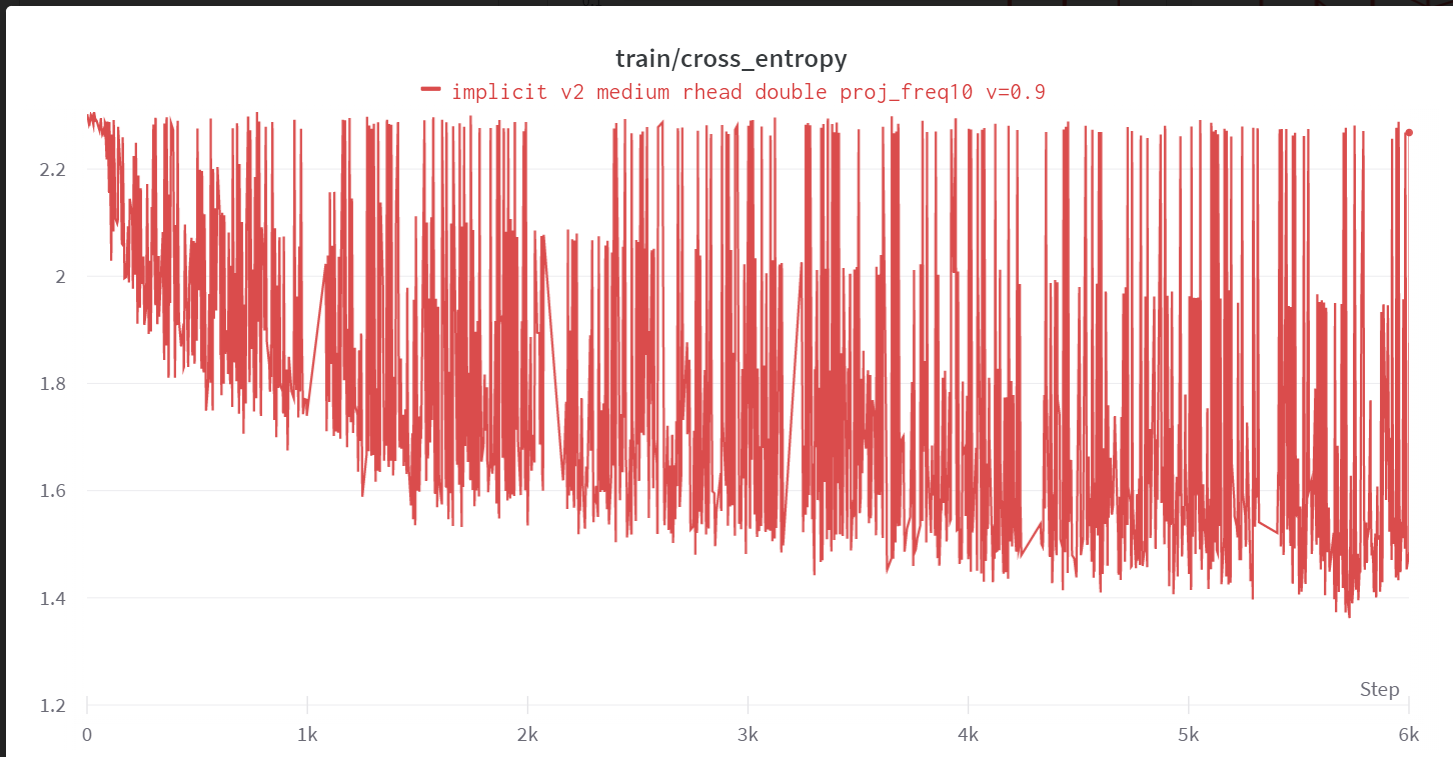
\includegraphics[width=0.8\linewidth]{images/implicit_v2_1.png}
\end{center}
Projection was done every 10 iterations, and as one can see each time the loss shoots back up to its initial value. 
$\nu$ was set to 0.9. A less destructive projection algorithm would be desirable.
\bibliographystyle{plainnat}
\bibliography{references}
\end{document}
